\section{Conclusion}

This paper focuses on the speaker name sensitivity in the text generation from dialogues. We provide a classification for previous approaches, and propose the insensitivity losses to reduce the sensitivity while achieving favorable generation quality. Fair comparisons and comprehensive analysis are done among different approaches for evaluating the sensitivity quantitatively. 
More approaches targeting dialogue sensitivity issues are expected.

\section*{Limitations}

Our work has the following limitations:

First, we cannot generalize our conclusions to other languages that are dramatically different from English or more complicated multi-lingual scenarios without further experiments.

Second, we didn't consider any special designs on demographic features of names in our proposed approach. As shown in Sec.~\ref{sec:unfairness}, discrimination does exist among different groups. Although Ins outperforms other baselines overall, there is still room to improve insensitivity among different groups for tasks with longer outputs containing multiple speaker names. We hypothesize that demographic features of names can be added through a more dedicated data augmentation strategy.

Third, our experimentation was restricted to the BART model in this paper. The reason is that among all the models that can be fine-tuned with our limited resources, including T5 and GPT-2, BART is still the best and the most popular, therefore we pick BART as the target of this study. Our intention is to devote the limited paper space to a more in-depth analysis of the problem using a range of tasks. Besides, it should be noticed that the speaker name sensitivity is still an issue with recent large pre-trained models, as shown in the example of dialogue summarization with outputs from ChatGPT in Fig.~\ref{fig:case-chatgpt}. The two summaries are expected to be the same, modulo speaker names. However, the third speaker (Sergio/Ashley) is not even mentioned in Summary-2.

\begin{figure}[h!]
	\centering
	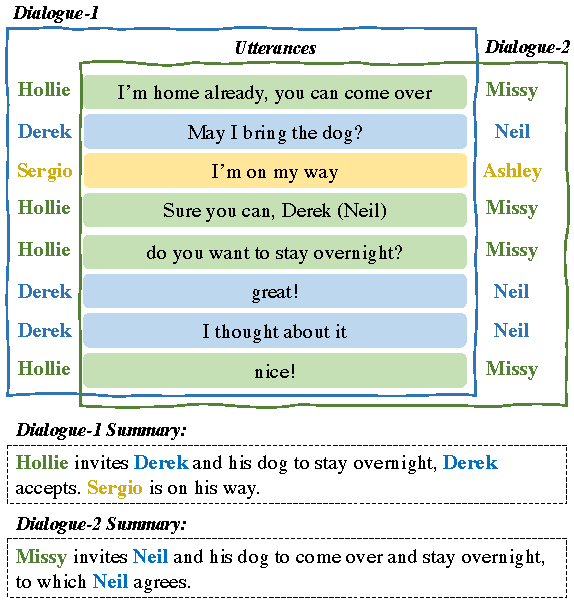
\includegraphics[width=0.95\linewidth]{case-chatgpt.pdf}
	\caption{An example of dialogue summarization with outputs from ChatGPT.} 
	\label{fig:case-chatgpt}
\end{figure}

We will try to address these limitations in the future.


\section*{Ethics Statement}

All of the name lists we adopted in this paper are borrowed from public websites (https://www.ssa.gov) and previous publications~\cite{tzioumis2018demographic, khalifa2021bag}. We considered only binary genders and four different racial groups, which are clearly incomplete for depicting all humans. Our work is mainly at drawing researchers' attention to the unfairness caused by speaker names in text generation tasks given dialogues. These demographic features are selected to shed light on this potential issue and our method is not restricted to any specific demographic groups.

